\problemname{Viðnámsflækja}
\illustration{0.3}{resistors}{Mynd fengin af \href{https://commons.wikimedia.org/wiki/File:Electronic-Axial-Lead-Resistors-Array.jpg}{commons.wikimedia.org}}

Eins og vanalega er allt í rugli hjá KFFÍ rétt fyrir keppni. Þegar aðrir fara að mæta út í HR til að aðstoða við að græja hluti er Bjarki þegar mættur, skríðandi undir borðum.
Aðspurður hvers vegna hann væri að þessu segist hann vera að laga snúruflækjur og tengja allt rétt saman svo hlutir virki. Hins vegar virðist eitthvað vera aðeins óvanalegt þar
sem margir vírnarnir eru farnir að hitna hættulega mikið. Vandinn er auðvitað viðnámið, hærra viðnám, meiri hiti. Meðan að Bjarki skríður undan borðinu og tekur sér pásu, gætir
þú fundið út úr því hvert viðnámið milli tveggja punkta í snúruflækjunni er?

Inntakið verður gefið sem samansafn punkta þar sem vírar mætast, ásamt vírum sem liggja milli þessarra punkta. Hver vír hefur eitthvað viðnám $n \Omega$, hér er $\Omega$ mælieiningin
Ohm. Einnig verða gefnir hvaða tveir punktar mæla á viðnámið á milli. Sem betur fer fyrir þig skildi einhver eðlisfræðinemi eftir glósurnar sínar í stofunni, svo þú hefur einhverjar
upplýsingar um hvernig skal reikna þetta.

Regla 1: Ef punktar $x, y$ hafa tvo ólíka víra á milli sín með viðnám $n \Omega$ og $m \Omega$ má skipta þeim báðum út fyrir einn vír með viðnám $1/(1/n+1/m) \Omega$.

\begin{figure}[h!]
  \centering
    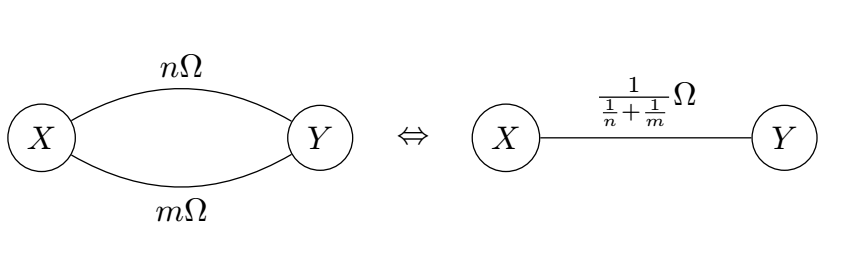
\includegraphics[width=0.5\textwidth]{regla1}
  \caption{Regla 1}
\end{figure}

Regla 2: Gerum ráð fyrir að til sé punktur $x$ sem er hvorki upphafs- né endapunktur. Gerum enn fremur ráð fyrir að $x$ sé tengdur með nákvæmlega einum vír í tvo ólíka aðra punkta $a, b$ sem hafa viðnám
$n \Omega$ og $m \Omega$. Þá má henda punktinum $x$ og í staðinn tengja $a$ og $b$ með vír með viðnám $(n + m)\Omega$. 

\begin{figure}[h!]
  \centering
    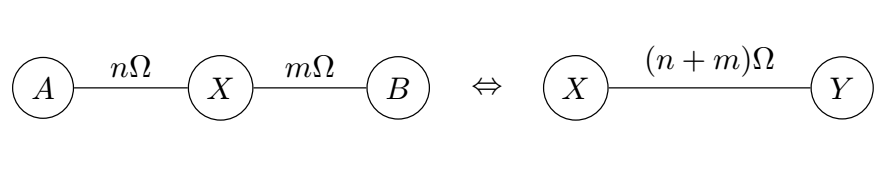
\includegraphics[width=0.5\textwidth]{regla2}
  \caption{Regla 2}
\end{figure}

Regla 3: Gerum ráð fyrir að til sé punktur $x$ sem er hvorki upphafs- né endapunktur. Gerum enn fremur ráð fyrir að $x$ sé tengdur með nákvæmlega einum vír í þrjá ólíka aðra punkta $a, b, c$ sem hafa viðnám
$n \Omega$, $m \Omega$ og $l \Omega$ í þeirri röð. Látum $s = (nm + nl + ml)$. Þá má henda punktinum $x$ og í staðinn tengja $a$ og $b$ með vír með viðnám $s/l \Omega$, tengja $a$ og $c$ með vír með viðnám
$s/m \Omega$ og tengja $b$ og $c$ með viðnám $s/n \Omega$. Einnig má framkvæma þessa breytingu afturábak.

\begin{figure}[h!]
  \centering
    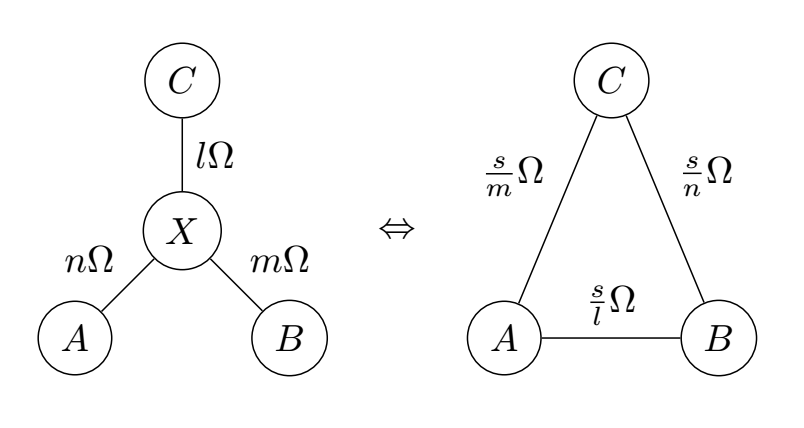
\includegraphics[width=0.5\textwidth]{regla3}
  \caption{Regla 3}
\end{figure}

\section*{Inntak}
Fyrsta lína inntaksins inniheldur tvær heiltölur $2 \leq n \leq 100$ og $1 \leq m \leq 10^5$, fjöldi punkta og fjöldi víra.
Næsta lína inniheldur tvær ólíkar heiltölur $1 \leq s, t \leq n$, upphafs- og endapunktur sem mæla á viðnám á milli.
Loks koma $m$ línur, hver með þremur heiltölum $1 \leq a, b \leq n$ og $1 \leq x \leq 1000$. $a, b$ eru ólík og gefa endapunkta vírsins en $x \Omega$ er viðnám vírsins.
Gefið er að alltaf sé einhver runa víra sem koma manni frá $s$ til $t$. Ef enginn einfaldur vegur frá $s$ til $t$ liggur um einhvern vír, þá má hunsa hann. Einfaldur vegur er leið frá $s$ til $t$ þar sem enginn vír kemur tvisvar fyrir.

\section*{Úttak}
Hægt er að sýna að svarið verði alltaf heiltölubrot. Segjum að svarið sé $p/q$ þar sem $p, q$ eru fullstytt. Þar sem $p, q$ geta orðið mjög stór á að prenta $pq^{-1} \pmod{10^9 + 7}$. Andhverfan 
er þá með tilliti til mátunarinnar (e. modulus).

\section*{Stigagjöf}
\begin{tabular}{|l|l|l|}
\hline
Hópur & Stig & Takmarkanir \\ \hline
1     & 30   & Aðeins þarf að beita reglu 1 til að fá svar. \\ \hline
2     & 30   & Aðeins þarf að beita reglu 2 til að fá svar. \\ \hline
3     & 30   & Aðeins þarf að beita reglum 1 og 2 til að fá svar. \\ \hline
4     & 10   & Aðeins þarf að beita reglum 1, 2 og 3 til að fá svar. \\ \hline
\end{tabular}

% Hópur 1 eru samanhangandi net á 2 hnútum
% Hópur 2 eru tré
% Hópur 3 er erfitt að lýsa betur en bara það sem stendur að ofan
% Hópur 4 eru lagnet án tengihnúta sbr Truemper, K. (1989). "On the delta-wye reduction for planar graphs". Journal of Graph Theory. 13 (2): 141–148. Má samt henda út öðrum blocks og ítra yfir blocks, so effektíft er þetta öll lagnet.
% En fyrir lokahópinn er auðveldara að nota aðferð sem virkar fyrir öll net.

\section*{Útskýring á sýnidæmum}
Fyrsta sýnidæmið fellur undir hóp 1. Svarið er $12/25$. $12 \cdot 25^{-1} \pmod{10^9 + 7}$ er $360000003$. Þetta er vegna þess að $360000003 \cdot 25 \equiv 12 \pmod{10^9 + 7}$. Tölurnar við hverja ör í skýringarmynd tákna hvaða reglu var beitt. \\

\begin{figure}[h!]
  \centering
    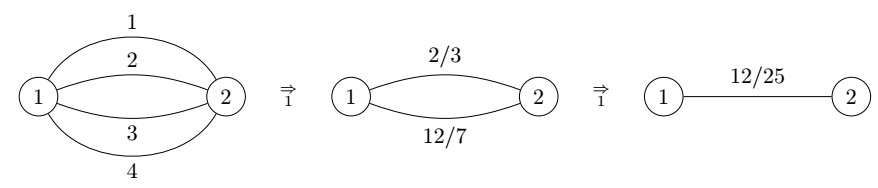
\includegraphics[width=0.5\textwidth]{sample1}
  \caption{Sýnidæmi 1}
\end{figure}

Annað sýnidæmið fellur undir hóp 2. Fyrsta örin merkt með $0$ táknar að verið sé að fjarlægja víra sem eru ekki hluti af neinum einföldum veg frá upphafs- til endapunkts. 

\begin{figure}[h!]
  \centering
    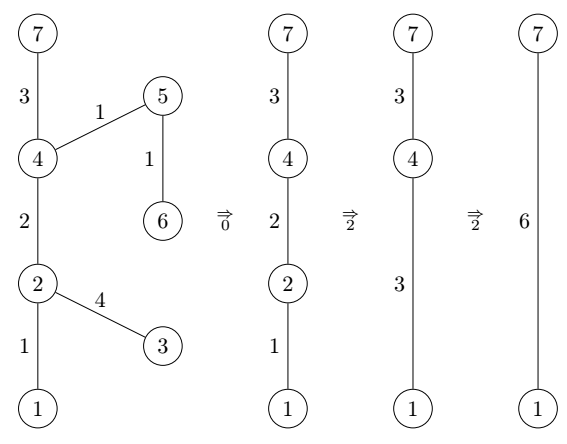
\includegraphics[width=0.5\textwidth]{sample2}
  \caption{Sýnidæmi 2}
\end{figure}

Þriðja sýnidæmið fellur undir hóp 3. Svarið er $20/11$. $20 \cdot 11^{-1} \pmod{10^9 + 7}$ er einmitt $363636368$. \\

\begin{figure}[h!]
  \centering
    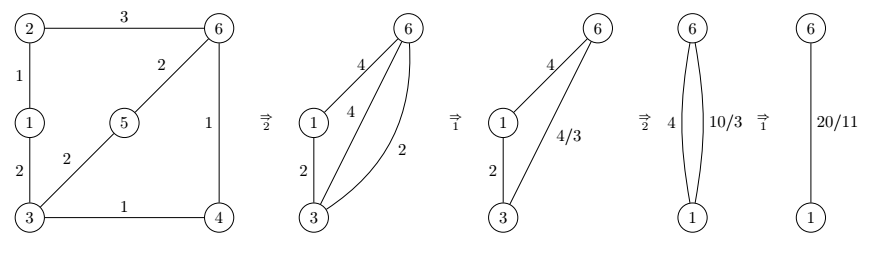
\includegraphics[width=0.5\textwidth]{sample3}
  \caption{Sýnidæmi 3}
\end{figure}

Fjórða sýnidæmið fellur undir hóp 4. Táknum með $3'$ þegar við notum reglu $3$ afturábak. Svarið er $5/6$, $5 \cdot 6^{-1} \pmod{10^9+7}$ er $833333340$. \\

\begin{figure}[h!]
  \centering
    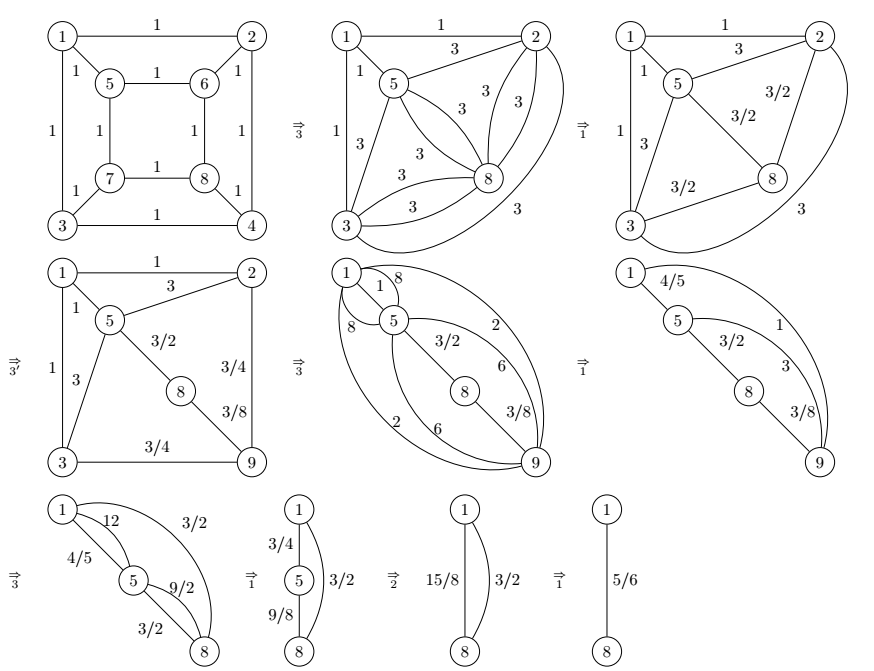
\includegraphics[width=0.5\textwidth]{sample4}
  \caption{Sýnidæmi 4}
\end{figure}
